\subsection{Análisis del Sistema de Disparo (Trigger y Nivel)}

El análisis del sistema de disparo se inicia conectando la señal sinusoidal de 50 Hz 5 Vrms del Generador de Funciones Rigol DG1022 al Canal 1 (CH1) del Osciloscopio Rigol DS4014. La ganancia vertical se ajusta a \SI{2.50}{\volt/div} y la base de tiempo a \SI{5.000}{ms/div}.

Como primera observación (Figura \ref{fig:trigger_ok}), se configura el trigger para sincronizar con la fuente en CH1, con un nivel (Level) fijado en \SI{0.00}{\volt} y seleccionando el flanco de subida (pendiente positiva). Bajo estas condiciones, se obtiene una traza perfectamente estable (estado "TD" - Triggered). Se comprueba visualmente que la forma de onda inicia su "dibujo" en el centro de la pantalla (el punto de disparo) exactamente cuando la señal cruza el nivel 0V con una pendiente positiva. Esto confirma el propósito fundamental del trigger: establecer un punto de referencia repetitivo para iniciar cada barrido horizontal, logrando que la forma de onda periódica aparezca fija.

\begin{figure}[H]
    \centering
    
\includegraphics[width=0.8\textwidth]{Newfile1.png}
    \caption{Señal sinusoidal (\SI{50}{\hertz}) estable en CH1. Configuración de trigger: Fuente CH1, Nivel = \SI{0.00}{\volt}, Pendiente Positiva.}
    \label{fig:trigger_ok}
\end{figure}

A continuación, se explora el efecto de variar el nivel de disparo (Level). Partiendo de la condición estable anterior (Figura \ref{fig:trigger_ok}), el nivel se varía lentamente hacia valores positivos. Durante este proceso, se observa cómo el punto de inicio de la traza se "desliza" hacia la derecha, subiendo por la pendiente de la onda sinusoidal. La señal, que originalmente partía en 0V, pasa a dibujarse desde puntos de voltaje cada vez más altos, dando la impresión visual de que la onda sinusoidal se transforma en una cosenoidal a medida que el nivel se acerca al máximo.

El resultado final de este barrido se muestra en la Figura \ref{fig:trigger_level_alto}. Al superar con el nivel de trigger (\SI{+7.55}{\volt}) la amplitud máxima de la señal, la condición de disparo (cruzar \SI{+7.55}{\volt} con pendiente positiva) nunca se cumple. En consecuencia, el osciloscopio deja de adquirir nuevas trazas y entra en estado \textbf{"WAIT"}, mostrando en pantalla la última señal que quedó almacenada en su memoria, tal como se predice en el marco teórico para el modo de disparo "Normal".

Se realiza el procedimiento análogo disminuyendo el nivel de trigger hacia valores negativos. La Figura \ref{fig:trigger_level_bajo} muestra el resultado con el nivel fijado en \SI{-7.00}{\volt}, un valor muy cercano al valle (amplitud mínima) de la señal. A diferencia del caso anterior, la señal se mantiene perfectamente estable (estado "TD" - Triggered), ya que el nivel de disparo, aunque bajo, sigue estando dentro del rango de voltaje de la señal [Vmin, Vmax]. Se concluye que si el nivel se hubiese ajustado por debajo del mínimo de la señal, el resultado habría sido idéntico al de la Figura \ref{fig:trigger_level_alto} (estado "WAIT").

\begin{figure}[H]
     \centering
     \begin{subfigure}[b]{0.48\textwidth}
         \centering
         
\includegraphics[width=\textwidth]{Newfile2.png}
         \caption{Estado "WAIT" al fijar el Nivel (\SI{+7.55}{\volt}) por encima del máximo de la señal.}
         \label{fig:trigger_level_alto}
     \end{subfigure}
     \hfill
     \begin{subfigure}[b]{0.48\textwidth}
         \centering
         
\includegraphics[width=\textwidth]{Newfile3.png}
         \caption{Señal estable al fijar el Nivel (\SI{-7.00}{\volt}) cerca del mínimo de la señal.}
         \label{fig:trigger_level_bajo}
     \end{subfigure}
        \caption{Efecto de ajustar el nivel de trigger (Level) fuera y dentro de los límites de amplitud de la señal.}
        \label{fig:trigger_level_fuera}
\end{figure}

Posteriormente, para analizar el efecto de la pendiente (\textit{Slope}), se conecta una señal triangular de \SI{50}{\hertz} al Canal 2 (CH2) y se configura el trigger para tener como fuente (Source) a dicho canal.
\begin{itemize}
    \item \textbf{Figura \ref{fig:trigger_slope_pos}:} Se configura el trigger con pendiente positiva y un nivel cercano a 0V. Se observa que ambas señales (sinusoidal en CH1 y triangular en CH2) están estables. La señal triangular (CH2, azul) inicia su traza en el centro de la pantalla (el punto de disparo) justo en el instante en que cruza el nivel de referencia con pendiente positiva (subiendo).
    
    \item \textbf{Figura \ref{fig:trigger_slope_neg}:} Se mantiene la misma configuración, pero se conmuta la pendiente a negativa (flanco de bajada). Nuevamente, ambas señales están estables, pero ahora la señal triangular (CH2, azul) inicia su traza en el centro cuando cruza el nivel de referencia con pendiente negativa (bajando).
\end{itemize}
Esta comparación confirma que la pendiente selecciona cuál de las dos intersecciones con el nivel de trigger se utiliza como punto de referencia, permitiendo estabilizar la imagen en el flanco de interés.

\begin{figure}[H]
     \centering
     \begin{subfigure}[b]{0.48\textwidth}
         \centering
         
\includegraphics[width=\textwidth]{Newfile4.png}
         \caption{Trigger en CH2 con pendiente positiva. La traza inicia cuando la señal azul (CH2) sube.}
         \label{fig:trigger_slope_pos}
     \end{subfigure}
     \hfill
     \begin{subfigure}[b]{0.48\textwidth}
         \centering
         
\includegraphics[width=\textwidth]{Newfile6.png}
         \caption{Trigger en CH2 con pendiente negativa. La traza inicia cuando la señal azul (CH2) baja.}
         \label{fig:trigger_slope_neg}
     \end{subfigure}
        \caption{Efecto de la selección de pendiente (Slope) del trigger (Fuente: CH2).}
        \label{fig:trigger_slope}
\end{figure}

Se realiza también la prueba de sincronización con la red eléctrica (Line) como fuente de trigger, volviendo a las señales de \SI{50}{\hertz} en CH1 y CH2. En esta configuración, no es posible lograr una sincronización completamente estable; las trazas de CH1 y CH2 se observan "desplazándose" lentamente en la pantalla. Esta inestabilidad se debe a que la frecuencia de la red eléctrica, aunque nominalmente es de \SI{50}{\hertz}, no es perfectamente constante y presenta fluctuaciones. En contraste, el generador de funciones Rigol DG1022 produce una señal de \SI{50.00}{\hertz} de alta precisión. La pequeña diferencia entre la frecuencia fija del generador y la frecuencia variable de la red eléctrica genera una diferencia de fase acumulativa que se manifiesta como un movimiento de la traza. Aunque se intentó ajustar manualmente la frecuencia del generador (ej., \SI{50.1}{\hertz} o \SI{49.91}{\hertz}) para igualar la de la red, la fluctuación inherente de esta última impidió una sincronización estática y duradera. Se concluye que, para el análisis de señales de laboratorio generadas con precisión, la sincronización con la red eléctrica no es una opción óptima.

Finalmente, se investiga el comportamiento al tener frecuencias distintas entre los canales, manteniendo la fuente de trigger fija en CH1 (sinusoidal, \SI{50}{\hertz}). La Figura \ref{fig:trigger_freq_distintas} muestra los resultados al variar la frecuencia de la señal triangular en CH2.

\begin{figure}[H]
     \centering
     \begin{subfigure}[b]{0.48\textwidth}
         \centering
         
\includegraphics[width=\textwidth]{Newfile7.png}
         \caption{Trigger en CH1 (\SI{50}{\hertz}), CH2 con $f_2 = \SI{100}{\hertz}$ ($2 \times f_1$). Ambas estables.}
         \label{fig:trigger_freq_multiplo}
     \end{subfigure}
     \hfill
     \begin{subfigure}[b]{0.48\textwidth}
         \centering
         
\includegraphics[width=\textwidth]{Newfile9.png}
         \caption{Trigger en CH1 (\SI{50}{\hertz}), CH2 con $f_2 = \SI{25}{\hertz}$ ($0.5 \times f_1$). CH2 inestable.}
         \label{fig:trigger_freq_submultiplo}
     \end{subfigure}
     \\ % Salto de línea para la siguiente imagen
     \vspace{1em} % Espacio vertical
     \begin{subfigure}[b]{0.48\textwidth}
         \centering
         
\includegraphics[width=\textwidth]{Newfile8.png}
         \caption{Trigger en CH1 (\SI{50}{\hertz}), CH2 con $f_2 = \SI{69}{\hertz}$ (no relacionada). CH2 inestable.}
         \label{fig:trigger_freq_no_relacionada}
     \end{subfigure}
        \caption{Efecto de la fuente de trigger (CH1) con frecuencias distintas en CH2.}
        \label{fig:trigger_freq_distintas}
\end{figure}


\begin{itemize}
    \item \textbf{Figura \ref{fig:trigger_freq_multiplo}:} La frecuencia de CH2 es de \SI{100}{\hertz}, un múltiplo entero ($2 \times$) de la frecuencia de trigger ($f_1 = \SI{50}{\hertz}$). Se observa que ambas señales se mantienen estables. Esto ocurre porque la relación de frecuencias es un número entero ($f_2 / f_1 = 2$). Cada vez que el osciloscopio se dispara en el mismo punto de la señal de CH1 (cada $T_1 = 20$ ms), la señal de CH2 ha completado exactamente 2 de sus propios ciclos ($T_2 = 10$ ms), por lo que también se encuentra en el mismo punto de su fase.
    
    \item \textbf{Figura \ref{fig:trigger_freq_submultiplo}:} La frecuencia de CH2 es de \SI{25}{\hertz}, un submúltiplo exacto ($1/2 \times$) de la frecuencia de trigger ($f_1 = \SI{50}{\hertz}$). En la captura estática, la señal de CH1 (trigger) aparece estable, pero la señal de CH2 (azul) se observa en movimiento. Esto se debe a que el trigger se activa cada $T_1 = 20$ ms, mientras que el periodo de CH2 es $T_2 = 40$ ms. El primer disparo ($t=0$) captura CH2 en un punto; el segundo disparo ($t=20$ ms) captura CH2 a la mitad de su ciclo; el tercer disparo ($t=40$ ms) captura a CH2 de vuelta en el punto original. Por lo tanto, el osciloscopio superpone dos trazas distintas para CH2, dando la apariencia de inestabilidad.
    
    \item \textbf{Figura \ref{fig:trigger_freq_no_relacionada}:} La frecuencia de CH2 se ajusta a \SI{69}{\hertz}, un valor no relacionado armónicamente con $f_1$. Como no se observa en la imagen, la señal de CH1 (trigger) permanece estable, pero la señal de CH2 (azul) se muestra completamente inestable, desplazándose erráticamente por la pantalla. El trigger se activa cada 20 ms, pero este intervalo no es un múltiplo racional simple del periodo de CH2 ($T_2 = 1/69 \text{ s} \approx 14.49$ ms). Por lo tanto, cada barrido captura la señal de CH2 en un punto de fase completamente diferente, haciendo imposible su análisis visual.
\end{itemize}

El análisis de estos casos permite establecer la condición de estabilidad para múltiples señales: para que dos señales (con $f_1$ como trigger) se vean estables, la frecuencia de la segunda señal ($f_2$) debe ser un múltiplo entero de la frecuencia de trigger ($f_2 = n \cdot f_1$). Si $f_2$ es un submúltiplo racional ($f_2 = (n/m) \cdot f_1$), la señal $f_2$ aparecerá estable solo si la base de tiempo total de la pantalla ($T_{\text{ventana}}$) se ajusta para ser un múltiplo común de ambos períodos ($T_1$ y $T_2$). Para frecuencias no relacionadas (irracionales o con relaciones racionales complejas como 69/50), la estabilidad visual es, en la práctica, imposible de lograr.




\subsection{Estudio de Acoplamientos y Modos de Visualización}

La Figura \ref{fig:11}] presenta la medición de las dos señales de entrada con el osciloscopio configurado en acoplamiento de Corriente Continua (CC). Este modo permite visualizar y medir las señales completas, incluyendo tanto su componente alterna (CA) como su componente de corriente continua (valor medio u offset).

El panel de mediciones automáticas del instrumento proporciona los valores requeridos para ambas trazas. Para el CH1 (amarilla), se registra un valor medio (Avg) de $3.930 \text{ V}$, un período de $20.00 \text{ ms}$ y un valor efectivo de $5.809 \text{ V}_{\text{rms}} $ (Per Vrms: RMS de un periodo).

Para el CH2 (azul), se mide un valor medio de $-298.0 \text{ mV}$, un período idéntico de $20.00 \text{ ms}$ y un valor efectivo de $2.122 \text{ V}_{\text{rms}}$.

Estos valores medidos en el instrumento fueron posteriormente validados mediante un análisis computacional en MATLAB sobre los datos exportados, utilizando la FFT para separar la componente de DC, la fundamental y los armónicos restantes, arrojando resultados consistentes con los reportados por el osciloscopio.

## Revisar: y ese analisis en matlab está aquí entre nosotros? 




\begin{figure}[H]
    \centering
    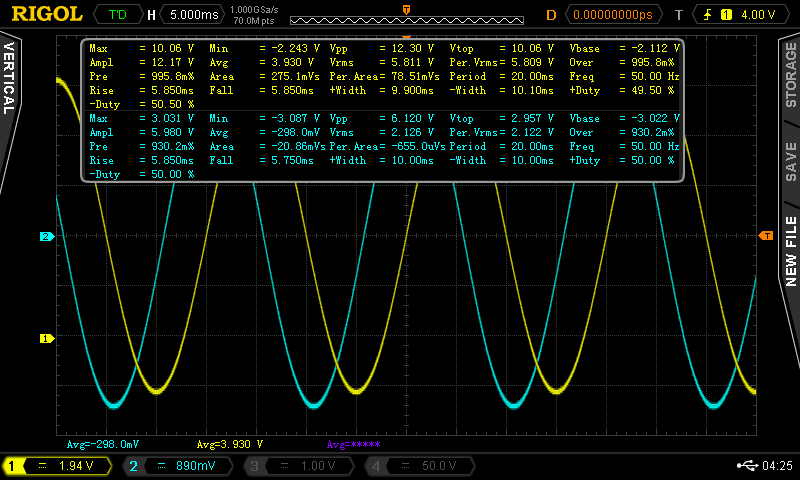
\includegraphics[width=0.8\linewidth]{NewDirectory1/Newfile1.png}
    \caption{(a) Acoplamiento CC y métricas para CH1 y CH2.}
    \label{fig:11}
\end{figure}




Utilizando los cursores del osciloscopio, se mide la diferencia de tiempo ($\Delta t$) entre puntos análogos de las dos formas de onda. En este caso, se han alineado los cursores con los cruces por cero con pendiente positiva de ambas señales. El panel de mediciones del instrumento, visible en la esquina superior izquierda, reporta una diferencia temporal $\Delta X = 4.480 \text{ ms}$.

Considerando que el período de ambas señales es $T = 20.00 \text{ ms}$ (correspondiente a la frecuencia de 50 Hz), el ángulo de desfase $\theta$ se calcula como:

$$ \theta = \frac{\Delta t}{T} \times 360^\circ = \frac{4.480 \text{ ms}}{20.00 \text{ ms}} \times 360^\circ = 80.64^\circ $$

Dado que el cruce de la señal del Canal 1 (amarilla) ocurre en un instante posterior (cursor B) que el del Canal 2 (cursor A), se concluye que la señal del Canal 1 se encuentra atrasada $80.64^\circ$ respecto a la señal del Canal 2.
\begin{figure}[H]
    \centering
    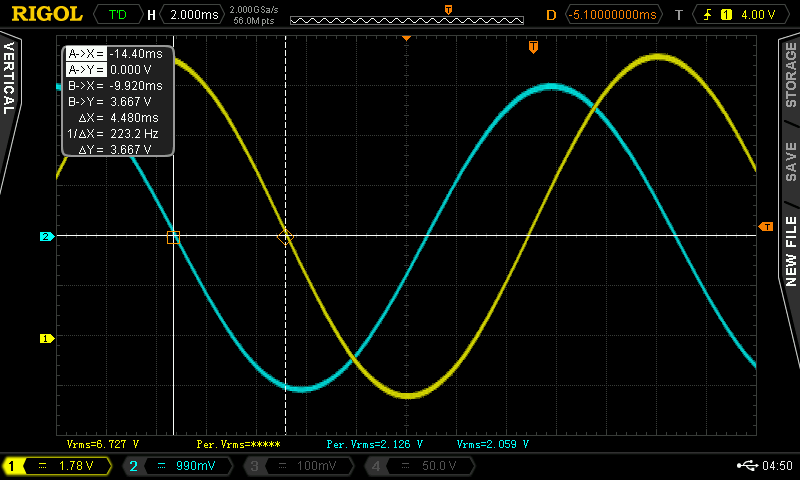
\includegraphics[width=0.5\linewidth]{NewDirectory1/Newfile3.png}
    \caption{(b) Medición de desfase entre CH1 y CH2 usando cursores, con acoplamiento CC.}
    \label{fig:13}
\end{figure}


A continuación, se coloca el osciloscopio en acoplamiento CA (Corriente Alterna) para verificar el desfase sin la influencia de los valores medios. La figura \ref{fig:aaaaaa} presenta esta medición. Se observa que ambas señales están ahora centradas en la referencia de $0 \text{ V}$, ya que sus respectivas componentes de CC han sido filtradas por el acoplamiento.

Utilizando nuevamente los cursores, se mide la diferencia temporal, arrojando un $\Delta X = -4.240 \text{ ms}$. Este valor corresponde a un ángulo de desfase de $\theta \approx 76.3^\circ$. Se destaca que cuando se hizo modo invertido para ambos canales, se mantuvo este valor.

Este resultado es notablemente similar al $\theta \approx 80.6^\circ$ obtenido en la medición con acoplamiento CC. La leve diferencia entre ambos valores se atribuye a la incertidumbre introducida por el posicionamiento manual de los cursores. Esto permite concluir y comprobar experimentalmente que la presencia de una componente de corriente continua (offset) en las señales no altera la relación de fase existente entre sus componentes armónicas.


\begin{figure}[H]
    \centering
    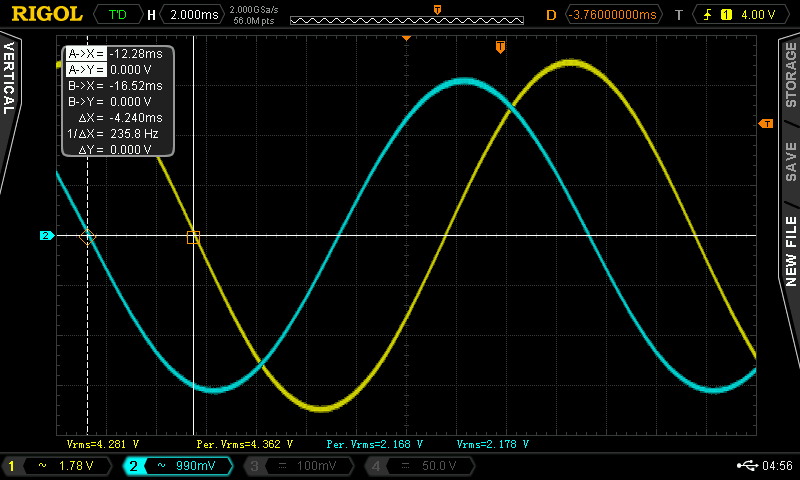
\includegraphics[width=0.5\linewidth]{NewDirectory1/Newfile4.png}
    \caption{(c) Medición de desfase con acoplamiento CA }
    \label{fig:aaaaaa}
\end{figure}



Finalmente, se selecciona el acoplamiento GND (Tierra) en los canales, cuyo resultado se observa en la Figura \ref{fig:gnd}. Al activar este modo, la señal de entrada se desconecta internamente y la entrada del amplificador vertical se conecta a la referencia de tierra del osciloscopio.

Como resultado, la pantalla muestra una línea horizontal perfectamente recta, indicando un nivel de tensión de $0 \text{ V}$. La utilidad principal de esta función es práctica, ya que permite al usuario verificar o ajustar con precisión la posición vertical que corresponde a la referencia cero en la pantalla, antes de realizar mediciones absolutas en modo CC.

\begin{figure}[H]
    \centering
    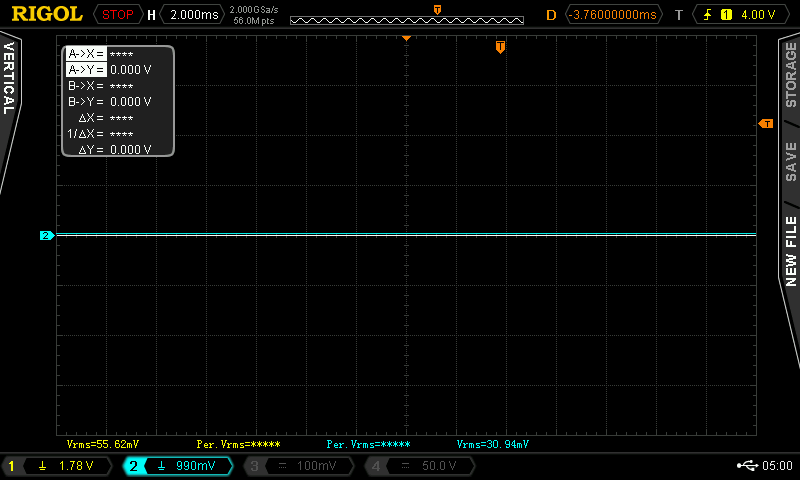
\includegraphics[width=0.5\linewidth]{NewDirectory1/Newfile5.png}
    \caption{(d) Acoplamiento GND}
    \label{fig:gnd}
\end{figure}

Se mantiene el acoplamiento CC, pero se activa el modo invertido en el Canal 1 (traza amarilla), tal como se observa en la Figura \ref{fig:einv}. Esta acción multiplica la señal de entrada del Canal 1 por $-1$, lo cual es matemáticamente equivalente a introducir un desfase adicional de $180^\circ$ a dicha señal.

El propósito es medir el nuevo desfase aparente. Al aplicar los cursores, el panel de medición reporta una diferencia temporal $\Delta X = -4.200 \text{ ms}$. El signo negativo indica que el punto de medición en el Canal 1 (Cursor B) ahora antecede al del Canal 2 (Cursor A), mostrando que el Canal 1 (invertido) lidera al Canal 2.

Este tiempo corresponde a un nuevo ángulo de desfase $\theta_{\text{nuevo}}$, calculado como:

$$ \theta_{\text{nuevo}} = \frac{4.200 \text{ ms}}{20.00 \text{ ms}} \times 360^\circ = 75.6^\circ $$

Este resultado es coherente con la teoría, que predice $\theta_{\text{nuevo}} = \theta_{\text{original}} + 180^\circ$. Tomando el desfase original medido de $\theta_{\text{original}} \approx 80.6^\circ$ (donde el Canal 1 estaba atrasado), el valor esperado sería $\theta_{\text{nuevo,teórico}} \approx -80.6^\circ + 180^\circ \approx +99.4^\circ$ (Canal 1 adelantado). La diferencia entre el valor teórico esperado y el valor medido se atribuye a las incertidumbres acumuladas en el posicionamiento manual de los cursores en ambas mediciones.

\begin{figure}[H]
    \centering
    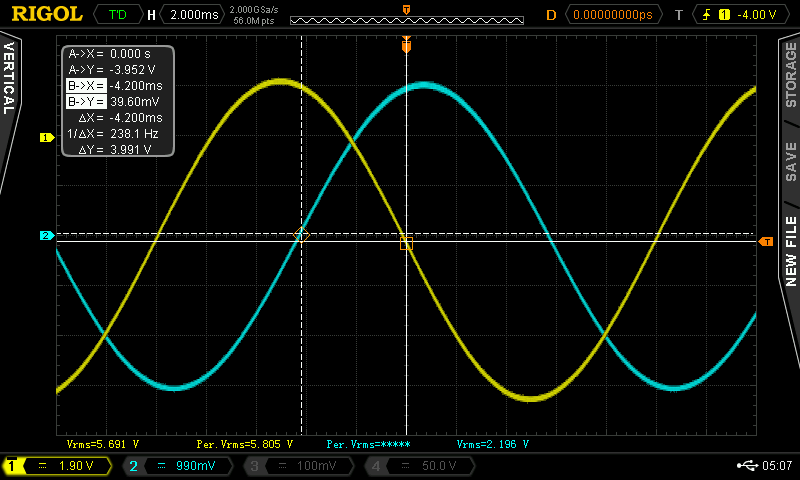
\includegraphics[width=0.5\linewidth]{NewDirectory1/Newfile6cchinv1.png}
    \caption{(e) Modo invertido para CH1 con acoplamiento CC}
    \label{fig:einv}
\end{figure}


\subsection{Análisis de Ganancias, Base de Tiempo y Modos Temporales}

\subsubsection{Modo Y-t}

Se configura el osciloscopio en su modo de operación principal Y-t, con el objetivo de optimizar la visualización de las señales. La Figura \ref{fig:2111} muestra la configuración inicial para las dos señales sinusoidales (CH1 en amarillo y CH2 en azul).

Para cumplir con el requisito de visualizar al menos dos ciclos, se ha seleccionado una base de tiempo de $5.000 \text{ ms/div}$. Considerando que las señales son de 50 Hz (período de $20.0 \text{ ms}$), esta escala permite desplegar 2.5 ciclos completos en la pantalla, satisfaciendo la condición. Las ganancias verticales se han ajustado a $5.00 \text{ V/div}$ para ambos canales, proporcionando una visualización clara de ambas formas de onda y estableciendo la referencia para las siguientes mediciones de amplitud.

\begin{figure}[H]
    \centering
    
\includegraphics[width=0.5\linewidth]{NewDirectory2/NewDirectory1/NewDirectory1/Newfile1.png}
    \caption{(1) Ajuste de ganancia y base de tiempo para tener al menos dos ciclos en pantalla.}
    \label{fig:2111}
\end{figure}

Siguiendo con el análisis de la ganancia, se procede a reducir la sensibilidad vertical del Canal 2, lo que implica aumentar su ajuste de Voltios por división (V/div). La Figura \ref{fig:imper} ilustra el resultado de este ajuste, donde la escala se ha fijado en $5.00 \text{ V/div}$.

A esta ganancia tan baja, la amplitud real de la señal del Canal 2 (que era de $1 \text{ V}_{\text{rms}}$) es significativamente menor que la resolución vertical representada por esta escala. Como consecuencia, la traza colapsa visualmente en una línea horizontal plana, volviéndose imperceptible e indistinguible del nivel de $0 \text{ V}$. Esto demuestra cómo un ajuste de ganancia inadecuado (una sensibilidad muy baja) puede ocultar completamente una señal que está activa y presente en la entrada.

\begin{figure}[H]
    \centering
    
\includegraphics[width=0.5\linewidth]{NewDirectory2/Newfile1.png}
    \caption{(2) Reducción de ganancia CH2 hasta que no se puede apreciar la señal.}
    \label{fig:imper}
\end{figure}

Se devuelve la ganancia a la configuración inicial, como estaba en la figura \ref{fig:2111} y luego se aumenta la ganancia de CH1 en un paso (en osciloscopio, un solo giro de perilla de CH1).

\begin{figure}[H]
    \centering
    
\includegraphics[width=0.5\linewidth]{NewDirectory2/NewDirectory1/NewDirectory1/Newfile2.png}
    \caption{(3) Aumento de ganancia en un paso para CH1.}
    \label{fig:step1}
\end{figure}


Se investiga el efecto opuesto al reducir progresivamente el ajuste de Voltios por división, aumentando así la ganancia. La Figura \ref{fig:2113} ilustra el resultado extremo de este ajuste, donde la ganancia se ha llevado a $1.00 \text{ mV/div}$ para ambos canales.

En esta condición de muy alta sensibilidad, las amplitudes reales de las señales ($5 \text{ V}_{\text{rms}}$ y $1 \text{ V}_{\text{rms}}$) exceden masivamente el rango dinámico vertical de la pantalla. Este fenómeno se conoce como saturación o ``clipping'', y se manifiesta visualmente como un recorte abrupto de las formas de onda. Las trazas aparecen como líneas horizontales planas en los límites superior e inferior del display. Es fundamental notar que, si bien esta configuración imposibilita por completo cualquier medición de amplitud o forma de onda, los cruces por cero aún son visibles, por lo que la medición de parámetros temporales, como el período, sigue siendo factible.
\begin{figure}[H]
    \centering
    
\includegraphics[width=0.5\linewidth]{NewDirectory2/NewDirectory1/NewDirectory1/Newfile3.png}
    \caption{(4) Aumento de ganancia para ambos canales hasta lograr saturación.}
    \label{fig:2113}
\end{figure}


% --- INICIO DEL CÓDIGO CORREGIDO PARA SECCIÓN 5.3.2 ---

\subsubsection{Modo X-Y y figura de Lissajous}

El osciloscopio se configura en modo X-Y. Este modo grafica la señal del Canal 2 (eje Y) en función de la señal del Canal 1 (eje X). La Figura \ref{fig:lissa_max_min} muestra la figura de Lissajous resultante para las dos señales de 50 Hz. En esta instancia, la figura toma la forma de una elipse casi alineada con los ejes, lo que sugiere un desfase cercano a los 90 grados.

El propósito de esta medición inicial es determinar los valores máximos de cada eje, los cuales representan las amplitudes pico de las señales. Para esto, se emplearon los cursores del osciloscopio. Como se observa en el panel de mediciones de la figura, los cursores se posicionaron en las extensiones máximas de la traza, arrojando los siguientes valores:

El eje X tiene valor máximo $V_{X,max} = 7.320 \text{ V}$ y valor mínimo $V_{X,min} = -7.240 \text{ V}$.

Para el eje Y los valores son $V_{Y,max} = 1.500\text{ V}$ y $V_{Y,min} = -1.440 \text{ V}$.

\begin{figure}[H]
    \centering
    % Asumo que la imagen 'Newfile3.png' de la carpeta NewDirectory2 es la correcta
    
\includegraphics[width=0.5\linewidth]{NewDirectory2/Newfile3.png} 
    \caption{Medición máximos y mínimos de cada eje usando cursores.}
    \label{fig:lissa_max_min} % Etiqueta corregida
\end{figure}

% Referencia a la figura correcta (\ref{fig:collage_principal_3x2})
La Figura \ref{fig:collage_principal_3x2} presenta la secuencia de las figuras registradas con el aumento de ángulo desfase del generador de señales (CH2). Se observa con claridad cómo la geometría de la traza evoluciona sistemáticamente con el ángulo de desfase $\phi$. Cerca de $\phi = 0^\circ$, la figura colapsa en una línea recta con pendiente positiva. A medida que el desfase aumenta a $30^\circ$, $45^\circ$ y $60^\circ$, la figura se abre progresivamente, formando una elipse inclinada que ocupa los cuadrantes I y III. Cuando el desfase alcanza exactamente $\phi = 90^\circ$, la elipse se alinea perfectamente con los ejes de la pantalla (convirtiéndose en un círculo si las amplitudes fuesen idénticas). Finalmente, al superar los $90^\circ$, como en el caso de $120^\circ$, la elipse cambia su orientación e inclinación, pasando a ocupar los cuadrantes II y IV. Este procedimiento comprueba de manera visual la dependencia directa entre la forma de la figura de Lissajous y el desfase temporal.

\begin{figure}[H] 
    \centering 
    
    % --- PRIMERA FILA ---
    % Sintaxis de subfigure corregida de [2.1] a [t] (top align)
    \begin{subfigure}[t]{0.45\textwidth} 
        \centering
        
\includegraphics[width=\textwidth]{NewDirectory2/NewDirectory1/Newfile1.png}
        \caption{Desfase 0$^\circ$}
        \label{fig:img1}
    \end{subfigure}
    \hfill % Espacio horizontal
    \begin{subfigure}[t]{0.45\textwidth}
        \centering
        
\includegraphics[width=\textwidth]{NewDirectory2/NewDirectory1/Newfile2.png}
        \caption{Desfase 30$^\circ$}
        \label{fig:img2}
    \end{subfigure}
    
    \vspace{5mm} % Espacio vertical entre filas
    
    % --- SEGUNDA FILA ---
    \begin{subfigure}[t]{0.45\textwidth}
        \centering
        
\includegraphics[width=\textwidth]{NewDirectory2/NewDirectory1/Newfile3.png}
        \caption{Desfase 45$^\circ$}
        \label{fig:img3}
    \end{subfigure}
    \hfill % Espacio horizontal
    \begin{subfigure}[t]{0.45\textwidth}
        \centering
        
\includegraphics[width=\textwidth]{NewDirectory2/NewDirectory1/Newfile4.png}
        \caption{Desfase 60$^\circ$}
        \label{fig:img4}
    \end{subfigure}
    
    \vspace{5mm} % Espacio vertical entre filas
    
    % --- TERCERA FILA ---
    \begin{subfigure}[t]{0.45\textwidth}
        \centering
        
\includegraphics[width=\textwidth]{NewDirectory2/NewDirectory1/Newfile5.png}
        \caption{Desfase 90$^\circ$}
        \label{fig:img5}
    \end{subfigure}
    \hfill % Espacio horizontal
    \begin{subfigure}[t]{0.45\textwidth}
        \centering
        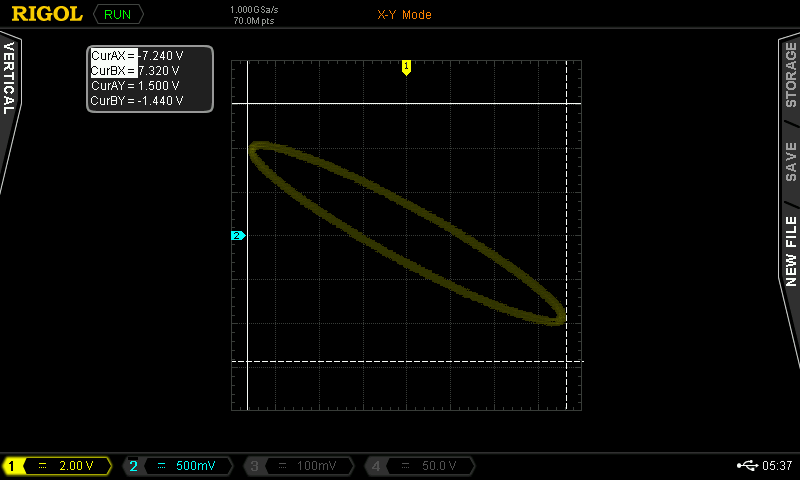
\includegraphics[width=\textwidth]{NewDirectory2/NewDirectory1/Newfile6.png}
        \caption{Desfase 120$^\circ$}
        \label{fig:img6}
    \end{subfigure}

    % --- LEYENDA PRINCIPAL ---
    \caption{Evolución de la figura de Lissajous con el incremento del desfase.}
    \label{fig:collage_principal_3x2}
\end{figure}

Se analiza el efecto de variar la relación de frecuencias entre los canales, manteniendo el osciloscopio en modo X-Y. Para este procedimiento, la señal del Canal 2 (eje X) se mantiene fija con una frecuencia $f_X = 50 \text{ Hz}$, mientras que la frecuencia de la señal del Canal 1 (eje Y), $f_Y$, se ajusta a diferentes múltiplos de 50 Hz.

\begin{figure}[H] 
    \centering 
    
    % --- IMAGEN 1 (FILA 1) ---
    % Sintaxis de subfigure corregida (eliminando [0.6\textwidth] innecesario)
    \begin{subfigure}{0.6\textwidth} 
        \centering
        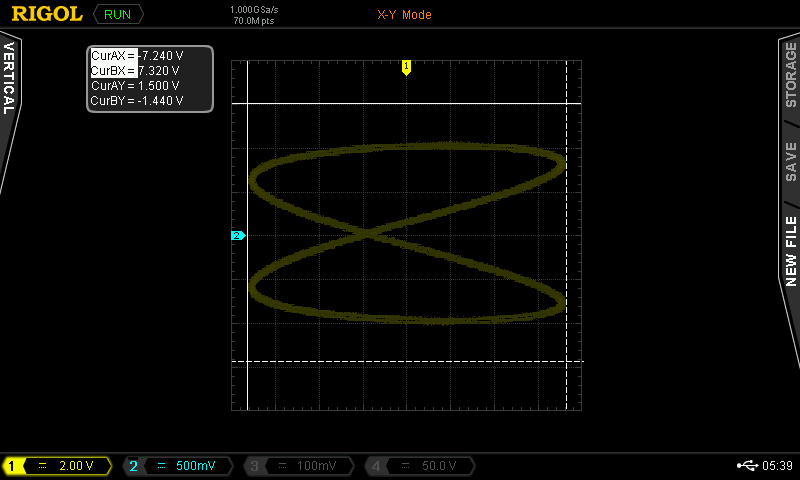
\includegraphics[width=\textwidth]{NewDirectory2/NewDirectory1/Newfile7.png}
        % Leyenda corregida (Análisis: 2 tangentes Y, 1 tangente X -> fY/fX = 2/1)
        \caption{Relación $f_Y / f_X = 2:1$ ($f_Y = \SI{100}{\hertz}$)}
        \label{fig:stack1}
    \end{subfigure}
    
    \vspace{5mm} % Espacio vertical entre imágenes
    
    % --- IMAGEN 2 (FILA 2) ---
    \begin{subfigure}{0.6\textwidth} 
        \centering
        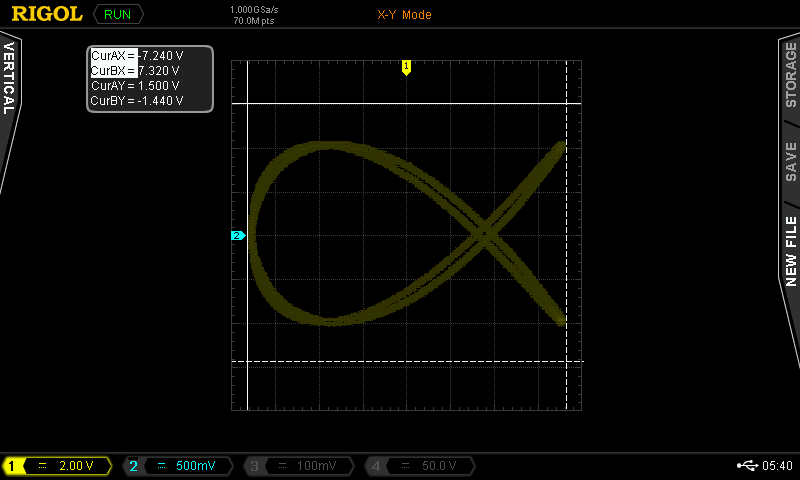
\includegraphics[width=\textwidth]{NewDirectory2/NewDirectory1/Newfile8.png}
        % Leyenda corregida (Análisis: 3 tangentes Y, 2 tangentes X -> fY/fX = 3/2)
        \caption{Relación $f_Y / f_X = 3:2$ ($f_Y = \SI{75}{\hertz}$)}
        \label{fig:stack2}
    \end{subfigure}
    
    \vspace{5mm} % Espacio vertical entre imágenes

    % --- IMAGEN 3 (FILA 3) ---
    \begin{subfigure}{0.6\textwidth} 
        \centering
        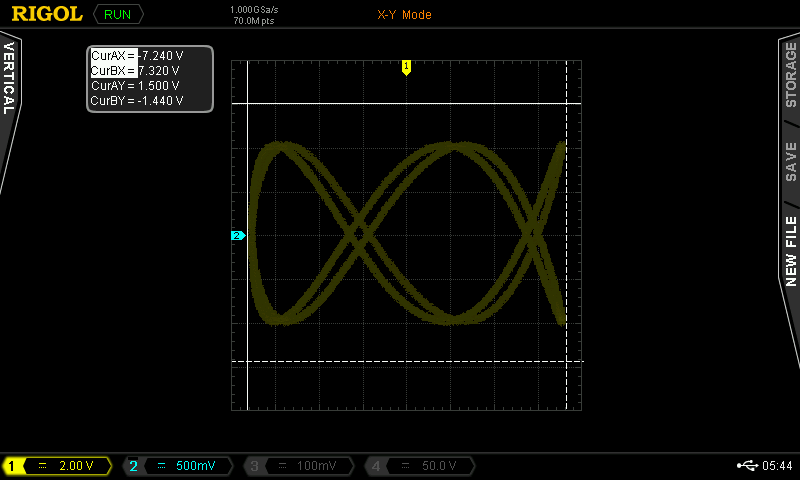
\includegraphics[width=\textwidth]{NewDirectory2/NewDirectory1/Newfile9.png}
        % Leyenda corregida (Análisis: 1 tangente Y, 2 tangentes X -> fY/fX = 1/2)
        \caption{Relación $f_Y / f_X = 1:2$ ($f_Y = \SI{25}{\hertz}$)}
        \label{fig:stack3}
    \end{subfigure}

    % --- LEYENDA PRINCIPAL ---
    % Leyenda principal corregida
    \caption{Figuras de Lissajous para distintas relaciones de frecuencia ($f_X = \SI{50}{\hertz}$).}
    \label{fig:lissa_mult}
\end{figure}

% --- FIN DEL CÓDIGO CORREGIDO ---


% Contenido para: sections/5datos.tex (Subsección 5.4)
\newpage
\subsection{Medición de Señal Transitoria}

La etapa final de la experiencia consistió en la captura y análisis de una señal transitoria no periódica, la cual, según se informó en el laboratorio, posee un flanco de subida muy rápido (aprox. \SIrange{2}{3}{\micro\second}) y un decaimiento exponencial lento (aprox. \SI{400}{\micro\second}). A diferencia de las mediciones anteriores con señales periódicas, este tipo de evento exige una configuración de disparo específica. Para lograr una captura estable, fue indispensable utilizar el modo de disparo \textbf{"Single"} del osciloscopio, el cual realiza un único barrido al cumplirse la condición de trigger y congela la traza en pantalla. El estado \textbf{"STOP"} visible en las Figuras \ref{fig:transitoria_completa} a \ref{fig:transitoria_bajada} confirma que el instrumento ha capturado exitosamente el evento.

Se realizaron tres mediciones con diferentes configuraciones de base de tiempo y trigger para analizar la señal en su totalidad, su flanco de subida y su flanco de bajada.

\subsubsection{Captura de la Señal Completa}
En la Figura \ref{fig:transitoria_completa}, se muestra la captura de la señal transitoria completa. Para lograr esto, se configuró una base de tiempo de \textbf{\SI{50.00}{\micro\second/div}}. Esto proporciona una ventana temporal total de \SI{500}{\micro\second} (10 divisiones), suficiente para capturar tanto la subida inicial como el decaimiento de \SI{400}{\micro\second}. El trigger se ajustó en el CH1 a un nivel de aproximadamente \SI{30}{\volt} con \textbf{pendiente positiva}, lo que permite iniciar la captura justo cuando el pulso comienza a ascender, capturando así el evento completo de forma efectiva.

\begin{figure}[H]
    \centering
    \begin{subfigure}[b]{0.48\textwidth}
        \centering
        
\includegraphics[width=\textwidth]{NewDirectory3/Newfile1.png}
        % --- Error corregido en \SI ---
        \caption{Captura del osciloscopio}
        \label{fig:transitoria_completa_osc}
    \end{subfigure}
    \hfill
    \begin{subfigure}[b]{0.48\textwidth}
        \centering
        % --- Ruta corregida ---
        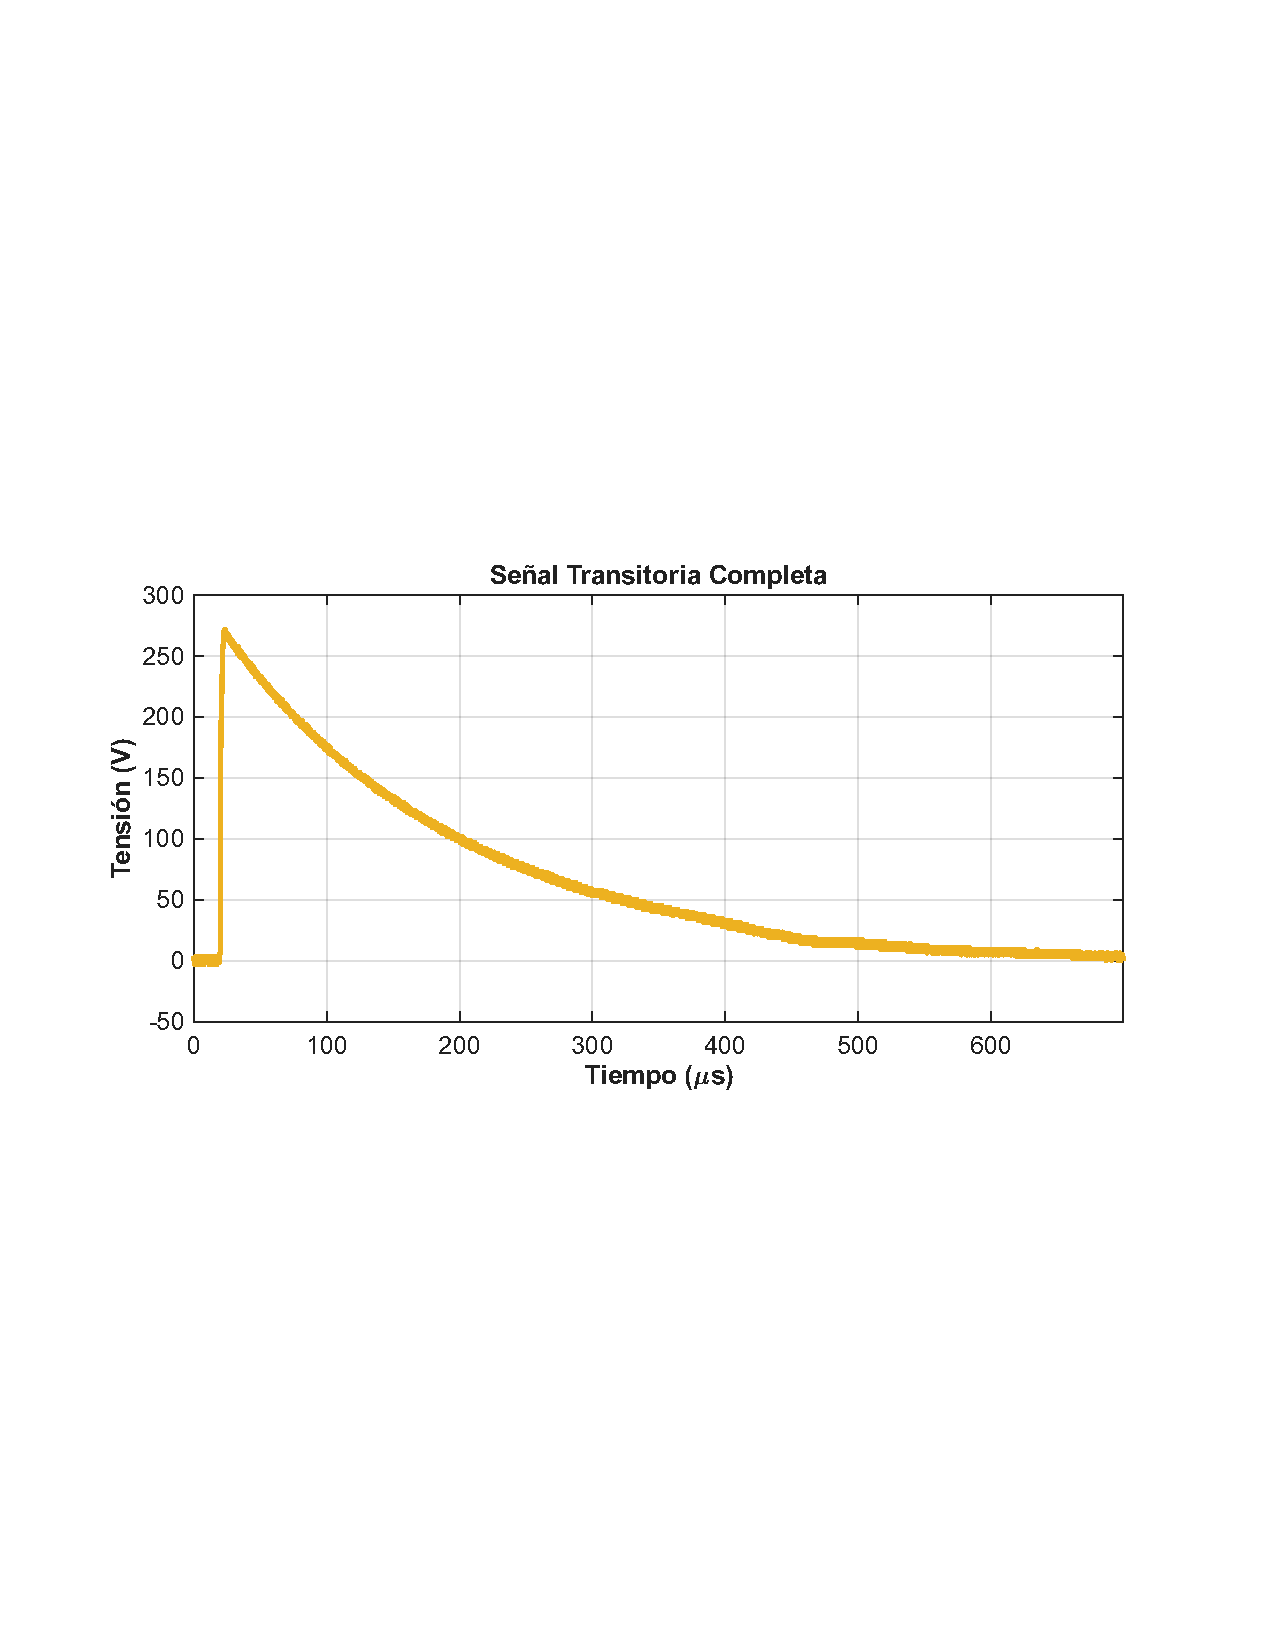
\includegraphics[width=\textwidth, trim={1cm 8cm 1cm 6cm}, clip]{NewDirectory3/Newfile1.pdf}
        \caption{Gráfico MATLAB}
        \label{fig:transitoria_completa_matlab}
    \end{subfigure}
    \caption{Visualización de la señal transitoria completa.}
    \label{fig:transitoria_completa}
% --- Error corregido de \beginAcronym ---
\end{figure}

\newpage
\subsubsection{Análisis del Flanco de Subida}
Para analizar en detalle el flanco de subida rápido, se redujo drásticamente la base de tiempo a \textbf{\SI{200.0}{ns/div}}, como se observa en la Figura \ref{fig:transitoria_subida}. Se mantuvo la configuración del trigger en CH1, con pendiente positiva y un nivel de \SI{30}{\volt}. Con esta ventana temporal tan estrecha (\SI{2}{\micro\second} en total), se logra capturar en todo su esplendor la evolución de la subida, mostrando cómo la señal pasa de su estado base a su valor máximo en un tiempo muy corto, coherente con los \SIrange{2}{3}{\micro\second} esperados.

\begin{figure}[H]
    \centering
    \begin{subfigure}[b]{0.48\textwidth}
        \centering
        
\includegraphics[width=\textwidth]{NewDirectory3/Newfile3.png}
        \caption{Captura del osciloscopio (\SI{200.0}{ns/div}).}
        \label{fig:transitoria_subida_osc}
    \end{subfigure}
    \hfill
    \begin{subfigure}[b]{0.48\textwidth}
        \centering
        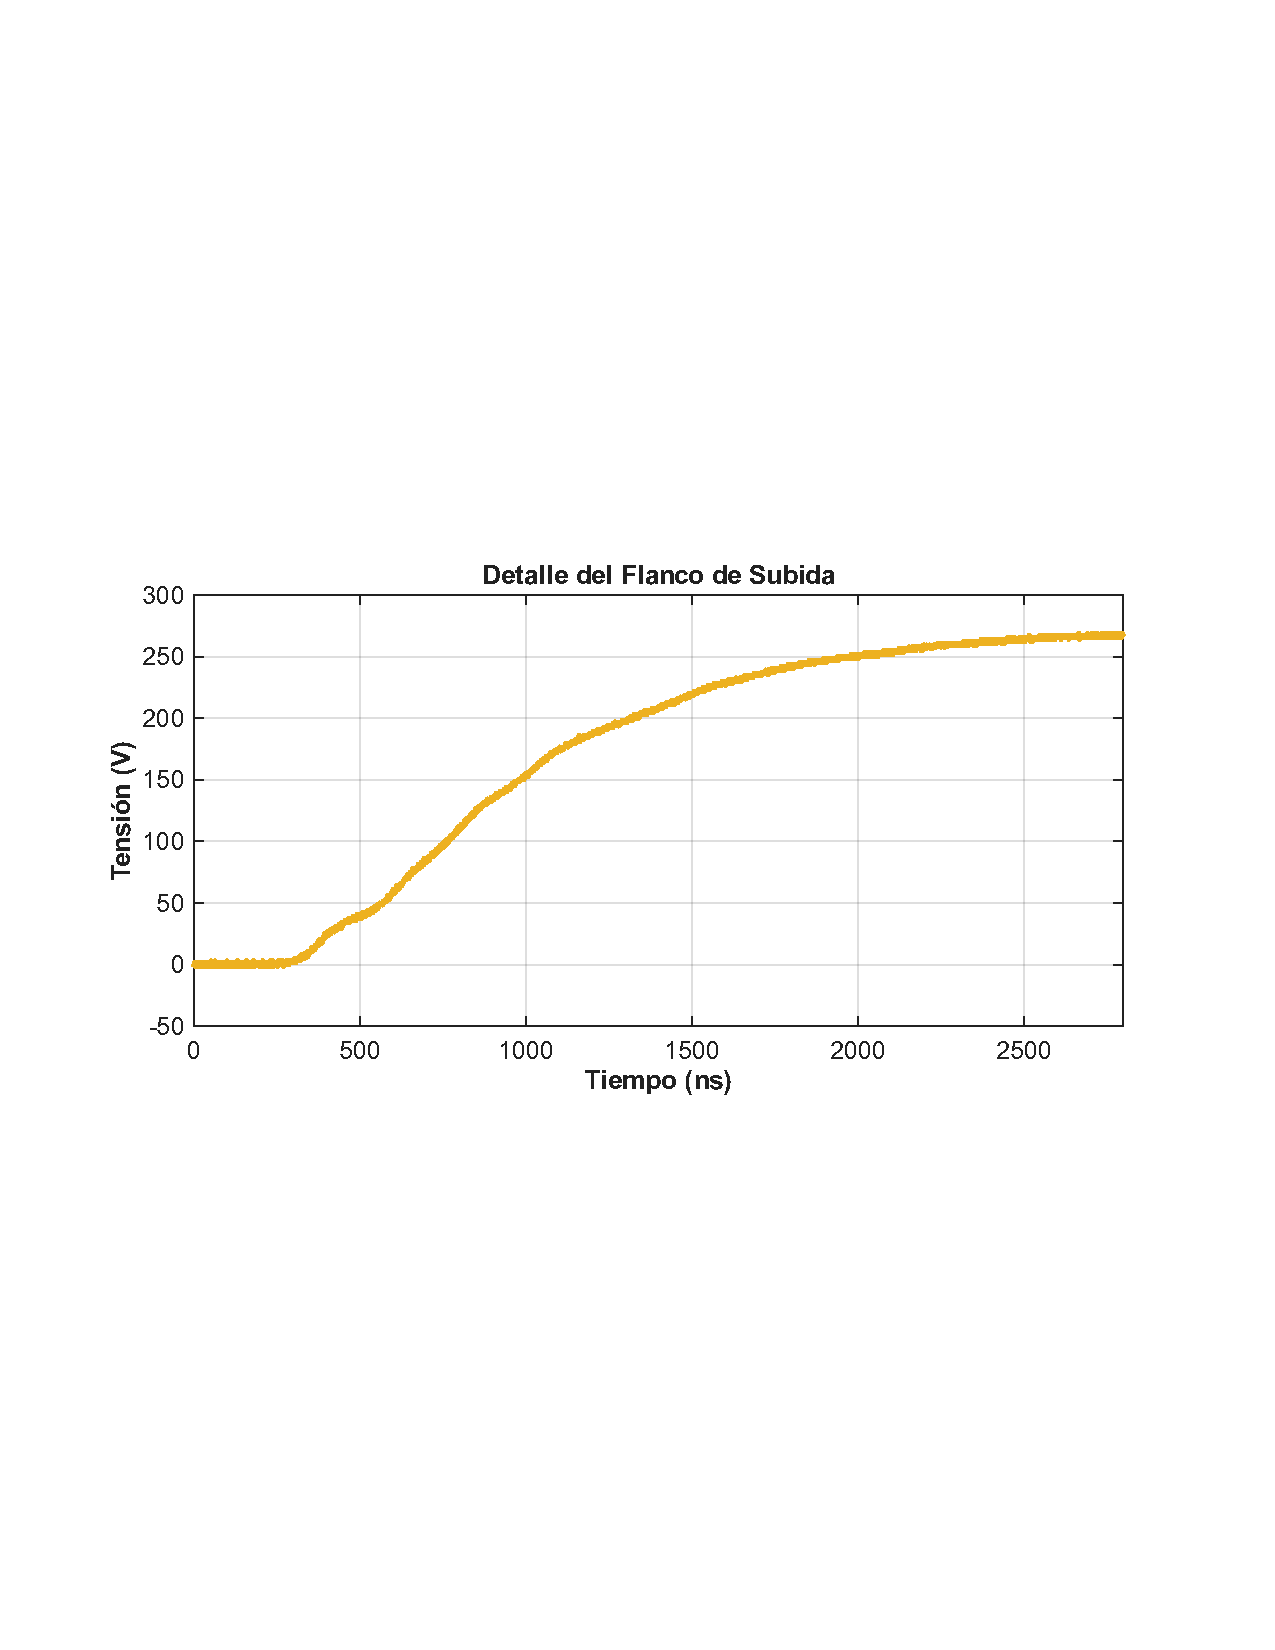
\includegraphics[width=\textwidth, trim={1cm 8cm 1cm 6cm}, clip]{NewDirectory3/Newfile3.pdf} % Asumiendo que el PDF se llama así
        \caption{Gráfico MATLAB}
        \label{fig:transitoria_subida_matlab}
    \end{subfigure}
    \caption{Análisis detallado del flanco de subida de la señal transitoria.}
    \label{fig:transitoria_subida}
\end{figure}

\subsubsection{Análisis del Flanco de Bajada}
Finalmente, se intentó capturar únicamente el flanco de bajada (decaimiento). Para esto, el trigger se configuró a un nivel de \SI{250}{\volt} con pendiente negativa, y la base de tiempo se ajustó a \textbf{\SI{10.00}{\micro\second/div}} (Figura \ref{fig:transitoria_bajada}). El análisis de esta captura revela que la medición no fue exitosa por dos razones principales:
\begin{enumerate}
    \item \textbf{Base de tiempo incorrecta:} La ventana temporal total es de \SI{100}{\micro\second} ($10 \text{ div} \times \SI{10}{\micro\second/div}$), lo cual es insuficiente para observar el decaimiento completo de \SI{400}{\micro\second}.
    \item \textbf{Posición del trigger:} El punto de trigger (indicado con \textbf{T}) está desplazado a la izquierda de la pantalla, pero no lo suficiente. Esto provoca que una importante porción de la pantalla capture el evento antes del disparo (el flanco de subida), fallando el objetivo de aislar únicamente la bajada y no se pudo repetir la medición por falta de tiempo en el laboratorio.
\end{enumerate}
Paradójicamente, la captura de la señal completa (Figura \ref{fig:transitoria_completa}) ofrece una mejor visualización del decaimiento.

Para una correcta medición del flanco de bajada, se debió haber configurado el osciloscopio de manera diferente: Aumentar la base de tiempo a \SI{50.00}{\micro\second/div} para tener una ventana de \SI{500}{\micro\second}, y ajustar la posición horizontal del trigger al extremo izquierdo de la pantalla. De esta forma, el disparo (pendiente negativa, \SI{310}{\volt}) iniciaría el barrido justo en el comienzo del decaimiento, utilizando toda la pantalla para graficar la bajada de la señal.

\begin{figure}[H]
    \centering
    \begin{subfigure}[b]{0.48\textwidth}
        \centering
        
\includegraphics[width=\textwidth]{NewDirectory3/Newfile4.png}
        \caption{Captura del osciloscopio (\SI{10.00}{\micro\second/div}).}
        \label{fig:transitoria_bajada_osc}
    \end{subfigure}
    \hfill
    \begin{subfigure}[b]{0.48\textwidth}
        \centering
        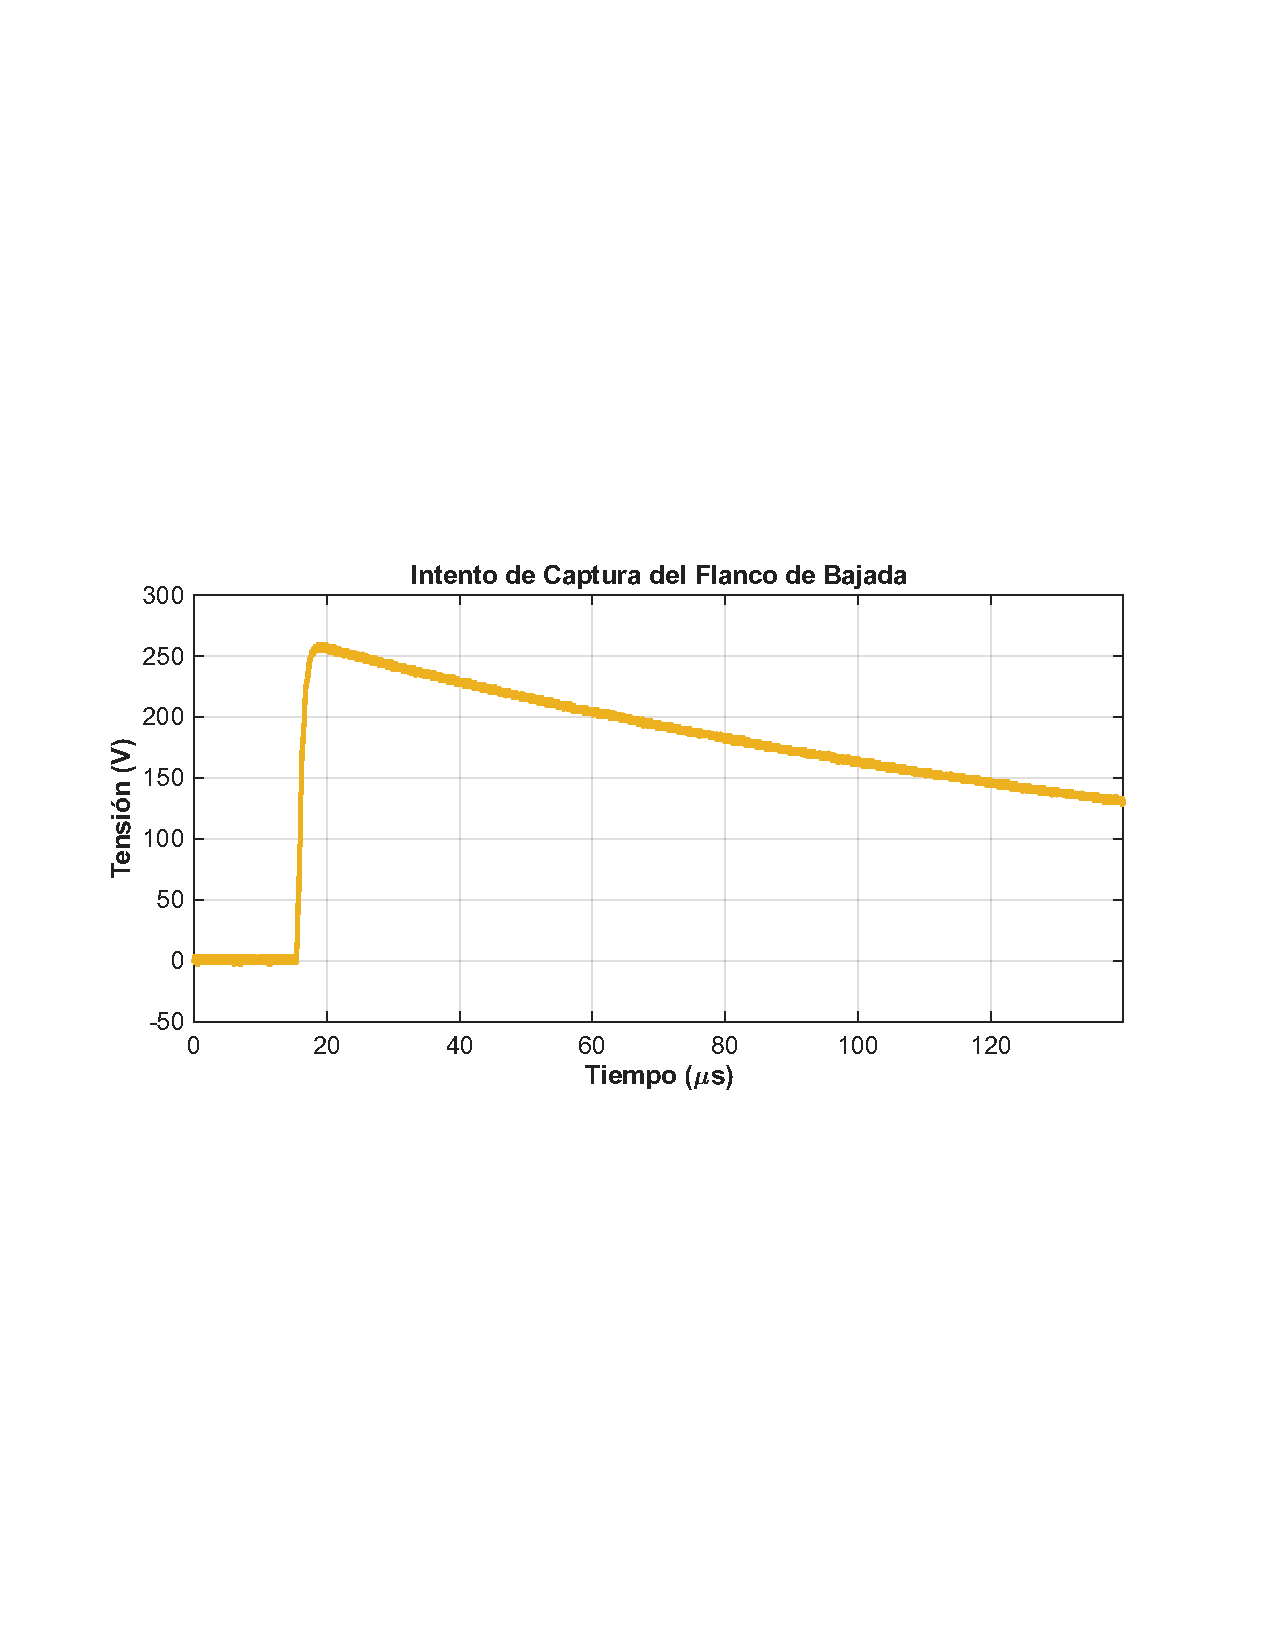
\includegraphics[width=\textwidth, trim={1cm 8cm 1cm 6cm}, clip]{NewDirectory3/Newfile4.pdf} % Asumiendo que el PDF se llama así
        \caption{Gráfico MATLAB}
        \label{fig:transitoria_bajada_matlab}
    \end{subfigure}
    \caption{Intento fallido de captura del flanco de bajada.}
    \label{fig:transitoria_bajada}
\end{figure}



